\section{はじめに} \label{sec:introduction}
%==============================================================%

本書は初めて領域気象気候モデル({\scalerm})
を利用するユーザー向けに解説したユーザーズガイドです。
気象気候ライブラリー\scalelib version \version に対応した説明を記載します。
現在、\scalelib を利用するため、領域モデル\scalerm と全球モデル\scalegm が
用意されていますが、後者は、力学コアの整備のみされています。
そのため、本版では、\scalerm の使い方についてのみ詳しく述べています。
\scalegm については、次版で詳しく記載される予定です。
\scalerm の使い方を通して、\scalelib を他のモデルからの呼び出す方法を
習得することも可能です。
第\ref{chap:overview}章で\scalelib の概要について、
第\ref{chap:install}章で必要な環境、およびインストール方法について説明します。
続いて、第\ref{chap:tutorial_ideal}章で基本的な操作方法、
第\ref{chap:tutorial_real}章で現実大気実験の実行方法について
簡単な例を示しながら説明します。
第\ref{chap:install}章から第\ref{chap:tutorial_real}章までは
ひと繋がりのチュートリアルとなっており、
\scalerm を初めて使うユーザーは一通り通読することをお勧めます。
第\ref{chap:basic_usel}章以降は、設定の変更、機能やツールの説明が記載されています。

%%%
本書中の不明点やお気づきの点がございましたら、SCALE user's メーリングリスト\\
 \verb|scale-user@riken.jp|までご連絡ください。



\subsection{\scalelib の特徴} \label{subsec:scale_feature}
%--------------------------------------------------------------%

\scalelib (Scalable Computing for Advanced Library and Environment)は
計算機を用いて気象・気候科学計算を行う上で、
研究を進めやすいように事前処理から数値計算、
解析に至るまですべての過程を網羅する数値計算ライブラリを
目指したソフトウェアである。下記に挙げるような特徴を持つ。
\begin{itemize}
\item \scalelib は、「BSD-2ライセンス」のもとオープンソースソフトウェア
として提供されており、商用、非商用に関わらず自由な利用・改変・再配布が可能である。
\item \scalelib には、\scalerm (SCALE-Regional Model)、
%SCALE-GM(SCALE-Global Model)
といった組み上げ済みの数値モデルが含まれている。
\item \scalelib には、次節で説明する様々なコンポーネントが導入されており、
必要に応じて取り替えることが可能である。
\item \scalelib で提供されている物理過程は、他の数値モデルへ組み込んで
使用することも可能である。
\end{itemize}

ライセンスの詳細は、トップディレクトリ直下の``\verb|scale/LICENSE|''のファイルに記述されている。
\scalelib の使用前に一読しておくこと。またSCALEのWebページにも説明が記載されているので必要に応じて
参照すること(\url{http://scale.aics.riken.jp/})。



\subsection{\scalerm の構成}  \label{subsec:sturcture_scale_rm}
%--------------------------------------------------------------%
現在、\scalelib には下記のコンポーネントが実装されている。
\scalerm ではすべてのコンポーネントが利用可能である。
詳細なモデル構成や差分化手法については、
\citet{scale_2015}、\citet{satoy_2015b}、
および\citet{nishizawa_2015}を参照されたい。\\


\noindent{\bf フレームワーク関係}
\begin{itemize}
 \item カーテシアン格子系(Cartesian Arakawa C-grid)
 \item MPI通信を用いた二次元領域分割
 \item 各種投影法(Map-projection \& Map-factors)
 \item ネスティングシステム(1-way:親→子のみ)
   \begin{itemize}
    \item オンライン実行(複数ドメインの計算を同時に実行)
    \item オフライン実行(外側ドメインの計算終了後に、その結果を用いて内側ドメインの計算を行う)
   \end{itemize}
 \item 複数事例一括実行 システム(バルクジョブシステム)
 \item CF 規約\footnote{\url{http:/cfconventions.org}}に基づく \netcdf ファイル I/O
   \begin{itemize}
   \item {\netcdf}3 または {\netcdf}4 形式
   \end{itemize}
 \item 外部データ読み込みによる初期値・境界値データ作成
   \begin{itemize}
    \item WRF-ARW\footnote{\url{http://www.wrf-model.org}}、
NICAM\footnote{\url{http://nicam.jp}}、
その他\grads \footnote{\url{http://cola.gmu.edu/grads/}}フォーマットでの入力に対応
   \end{itemize}
\end{itemize}

{\bf 力学コア関係}
\begin{itemize}
 \item 方程式系: 3次元完全圧縮非静力学方程式系
 \item 数値解法: 陽解法と陰解法の両方を実装
   \begin{itemize}
    \item 水平陽解鉛直陽解法(HE-VE:Horizontally Explicit and Vertically Explicit method)
    \item 水平陽解法-鉛直陰解法(HE-VI:Horizontally Explicit and Vertically Implicit method)
%    \item HI-VI(陰解法)
   \end{itemize}
 \item 空間差分:
    \begin{itemize}
      \item 2次中央差分(2nd order central difference scheme)
      \item 4次中央差分(4th order central difference scheme)
      \item 6次中央差分(6th order central difference scheme)
      \item 3次風上差分(3rd order upwind difference scheme)
%      \item 3次風上差分(Koren(1993)filterあり)(3rd order upwind difference scheme with \citet{Koren_1993} filter)
      \item 5次風上差分(5-th order upwind difference scheme)
    \end{itemize}
 \item 時間差分:(詳細は、\citet{scale_2015}を参照のこと)
    \begin{itemize}
      \item 3次ルンゲクッタスキーム(Heun's 3rd order Runge-Kutta scheme)
      \item Wicker and Skamarock (2002)'s 3段ルンゲクッタスキーム \citep[3-step Runge-Kutta scheme of ][]{Wicker_2002}
      \item 4次ルンゲクッタスキーム(4th order Runge-Kutta scheme)
    \end{itemize}
 \item 非負保証:
    \begin{itemize}
      \item フラックス修正法(Flux Corrected Transport)
      \item Koren (1993)フィルター \citep{Koren_1993} (3次風上差分スキーム使用時のみ)
    \end{itemize}
 \item 数値フィルター: 4次超粘性・拡散(4-th order hyper-viscosity/diffusion)
 \item 地形: 地形に沿った座標系(Terrain following coordinate)
\end{itemize}


{\bf 物理過程}
\begin{itemize}
 \item 乱流過程: 複数から選択可能
   \begin{itemize}
    \item Smagorinsky-Lilly 型のサブグリッドモデル \citep{smagorinsky_1963,lilly_1962,Brown_etal_1994,Scotti_1993}
    \item Deardorff(1980) サブグリットモデル \citep{Deardorff_1980}
    \item MYNN2.5境界層モデル \citep{my_1982,nakanishi_2004}
   \end{itemize}
 \item 雲微物理: 複数から選択可能
   \begin{itemize}
    \item 3-class single momoent バルクモデル\citep{kessler_1969}
    \item 6-class single moment バルクモデル \citep{tomita_2008}
    \item 6-class double moment バルクモデル \citep{sn_2014}
    \item ビン法雲モデル \citep{suzuki_etal_2010}
   \end{itemize}
 \item 放射過程: k分布ベース放射スキーム\citep{sekiguchi_2008}
 \item 地表面モデル
  \begin{itemize}
   \item 陸面モデル: 熱拡散・バケツモデル
   \item 海洋モデル: 初期値固定・外部入力(時間変化あり)・スラブモデル
   \item 都市モデル: 単層キャノピーモデル \citep{kusaka_2001}
   \item バルク交換係数(陸面および海面): 普遍関数によるバルク法\citep{beljaars_1991,wilson_2001}もしくは Louis 型バルク法\citep{uno_1995}
  \end{itemize}
\end{itemize}

上記に加え、\scalerm のコンポーネントとして、
現実事例の計算に必要な地形や土地利用データを作成するツール、
理想実験の初期値・境界値、もしくは外部モデルから初期値・境界値を作成するツールが提供されている。

次節で\scalelib の思想とモデルの関係について説明するが、
\scalerm の実行とは直接関係ないため、
必要なければ読み飛ばしても構わない。


\subsection{\scalelib のライブラリとモデル} \label{subsec:scalelib_model}

\begin{figure}[htb]
\begin{center}
  
\includegraphics[width=0.9\hsize]{./figure/library.eps}\\
  \caption{\scalelib のねらい}
  \label{fig:scale}
\end{center}
\end{figure}

\scalelib は、理化学研究所 計算科学研究機構(RIKEN AICS)を中心に
開発が進められている気象・気候科学計算向けのライブラリである。
図 \ref{fig:scale}に\scalelib の思想の概念図を示す。
この図に示されるような諸問題に対応することを目指している。
\scalelib は次世代のスーパーコンピュータから小型PCクラスターに至るまで
広く用いられる事を念頭において開発されており、
気候・気象科学を専門とする科学者と計算機科学を専門とする科学者が
共同で開発を行っている。
そのため、スーパーコンピュータ「京」や富士通FX10等の
スーパーコンピュータに加え、インテル機のような汎用計算機でも
高い計算効率がでるように設計されている。
ユーザーには、スーパーコンピュータ「京」を
はじめとする並列計算機に対してチューニングされた
モデルコンポーネントや解析システム、テストセットなどを
提供する。


\scalelib を利用した数値モデルとして、
\scalerm が含まれている(図 \ref{fig:scale-rm})。
格子系、力学コア、各種物理過程などの基本的なコンポーネントは
\scalelib が提供する。
\scalerm は、予報変数などを配列を持ち、
\scalelib のコンポーネントを適切に呼び出すことで時間発展計算を行っている。
ユーザーは、必要に応じて、各コンポーネントを選択し、
組み合わせて使用することが可能である。


\begin{figure}[hbt]
\begin{center}
  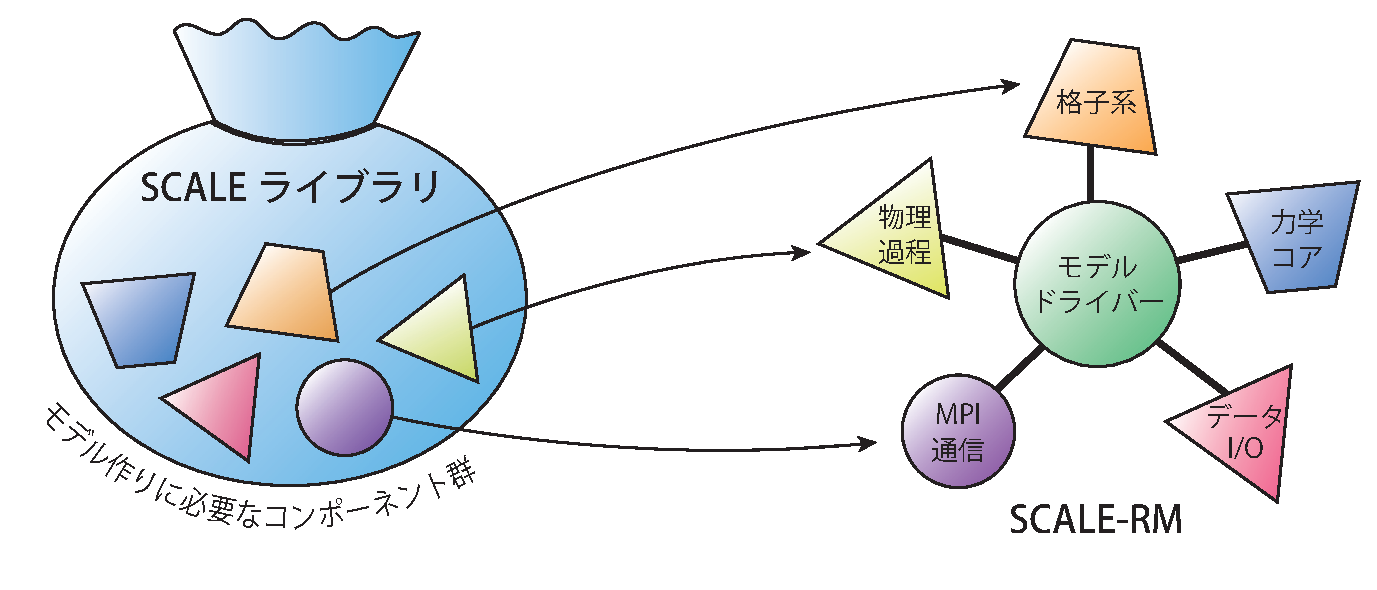
\includegraphics[width=0.9\hsize]{./figure/scale.eps}\\
  \caption{SCALEとSCALE-RMの関係}
  \label{fig:scale-rm}
\end{center}
\end{figure}


